
\section{Introduction}
Ce chapitre est consacré à la spécification des besoins de la plateforme StageFlow. Nous commençons par identifier les différents acteurs du système, puis nous détaillons les besoins fonctionnels et non fonctionnels. Enfin, nous présentons les diagrammes de cas d'utilisation et le diagramme de contexte.

\section{Identification des acteurs}
Un acteur est une entité externe qui interagit avec le système. Dans le cadre de StageFlow, nous avons identifié les acteurs suivants :

\begin{center}
\begin{tabular}{|l|p{10cm}|}
\hline
\textbf{Acteur} & \textbf{Description} \\ \hline
\textbf{Candidat} & Personne externe souhaitant postuler pour un stage. Il peut soumettre une candidature en ligne et suivre son état d'avancement. \\ \hline
\textbf{Admin RH} & Responsable des ressources humaines. Il gère l'ensemble du processus : validation des candidatures, affectation des stagiaires, génération des conventions et suivi global. \\ \hline
\textbf{Tuteur} & Encadrant assigné à un ou plusieurs stagiaires. Il suit leur présence quotidienne et rédige les évaluations de fin de stage. \\ \hline
\textbf{Stagiaire} & Candidat accepté et converti en stagiaire actif. Il consulte son espace personnel, son planning et ses évaluations. \\ \hline
\textbf{Services Externes} & Systèmes tiers utilisés par la plateforme : serveur SMTP pour l'envoi d'emails et SMS API pour les notifications. \\ \hline
\end{tabular}
\captionof{table}{Identification des acteurs du système StageFlow}
\end{center}

\section{Besoins fonctionnels}
Les besoins fonctionnels décrivent les fonctionnalités que le système doit fournir à ses utilisateurs.

\subsection{Besoins fonctionnels du Candidat}
\begin{itemize}
    \item Créer un compte avec vérification par email (OTP).
    \item Soumettre une candidature (CV + lettre de motivation).
    \item Suivre l'état de sa candidature en temps réel via un code de suivi.
\end{itemize}

\subsection{Besoins fonctionnels de l'Admin RH}
\begin{itemize}
    \item Consulter le tableau de bord avec les statistiques globales.
    \item Gérer les candidatures (accepter, refuser, mettre en attente).
    \item Convertir un candidat accepté en stagiaire.
    \item Affecter un stagiaire à un département et un tuteur.
    \item Générer automatiquement les conventions de stage en PDF.
    \item Gérer les départements de l'entreprise (CRUD).
    \item Consulter et exporter les rapports de présence.
    \item Gérer les utilisateurs et leurs rôles.
\end{itemize}

\subsection{Besoins fonctionnels du Tuteur}
\begin{itemize}
    \item Consulter la liste des stagiaires assignés.
    \item Saisir et valider les présences quotidiennes.
    \item Rédiger les évaluations de fin de stage.
    \item Recevoir des notifications concernant ses stagiaires.
\end{itemize}

\subsection{Besoins fonctionnels du Stagiaire}
\begin{itemize}
    \item Accéder à son espace personnel (dates de stage, département, tuteur).
    \item Consulter son historique de présence.
    \item Consulter ses évaluations.
    \item Télécharger ses documents (convention, attestation).
\end{itemize}

\section{Besoins non fonctionnels}
Les besoins non fonctionnels définissent les contraintes et les qualités attendues du système.

\begin{center}
\begin{tabular}{|l|p{10cm}|}
\hline
\textbf{Catégorie} & \textbf{Description} \\ \hline
\textbf{Sécurité} & Hachage des mots de passe avec Bcrypt, authentification par JWT, contrôle d'accès par rôles (RBAC), vérification OTP par email. \\ \hline
\textbf{Performance} & Temps de réponse inférieur à 2 secondes pour les opérations courantes, gestion d'un pool de 10 connexions MySQL simultanées. \\ \hline
\textbf{Ergonomie} & Interface intuitive et responsive, compatible avec les navigateurs modernes (Chrome, Firefox, Edge) et les appareils mobiles. \\ \hline
\textbf{Fiabilité} & Protection contre les attaques par force brute (Rate Limiting), sécurisation des en-têtes HTTP (Helmet), journalisation des requêtes. \\ \hline
\textbf{Maintenabilité} & Code structuré selon le pattern MVC, séparation claire Frontend/Backend, utilisation d'un ORM pour l'abstraction de la base de données. \\ \hline
\textbf{Disponibilité} & Le système doit être accessible en permanence pendant les heures de travail avec un taux de disponibilité de 99\%. \\ \hline
\end{tabular}
\captionof{table}{Besoins non fonctionnels de StageFlow}
\end{center}

%%% --- IMAGE : Besoins non fonctionnels ---
%%% Remplacer IMAGE_BESOINS_NON_FONCTIONNELS.png par le nom de ton image
% \begin{figure}[H]
%     \centering
%     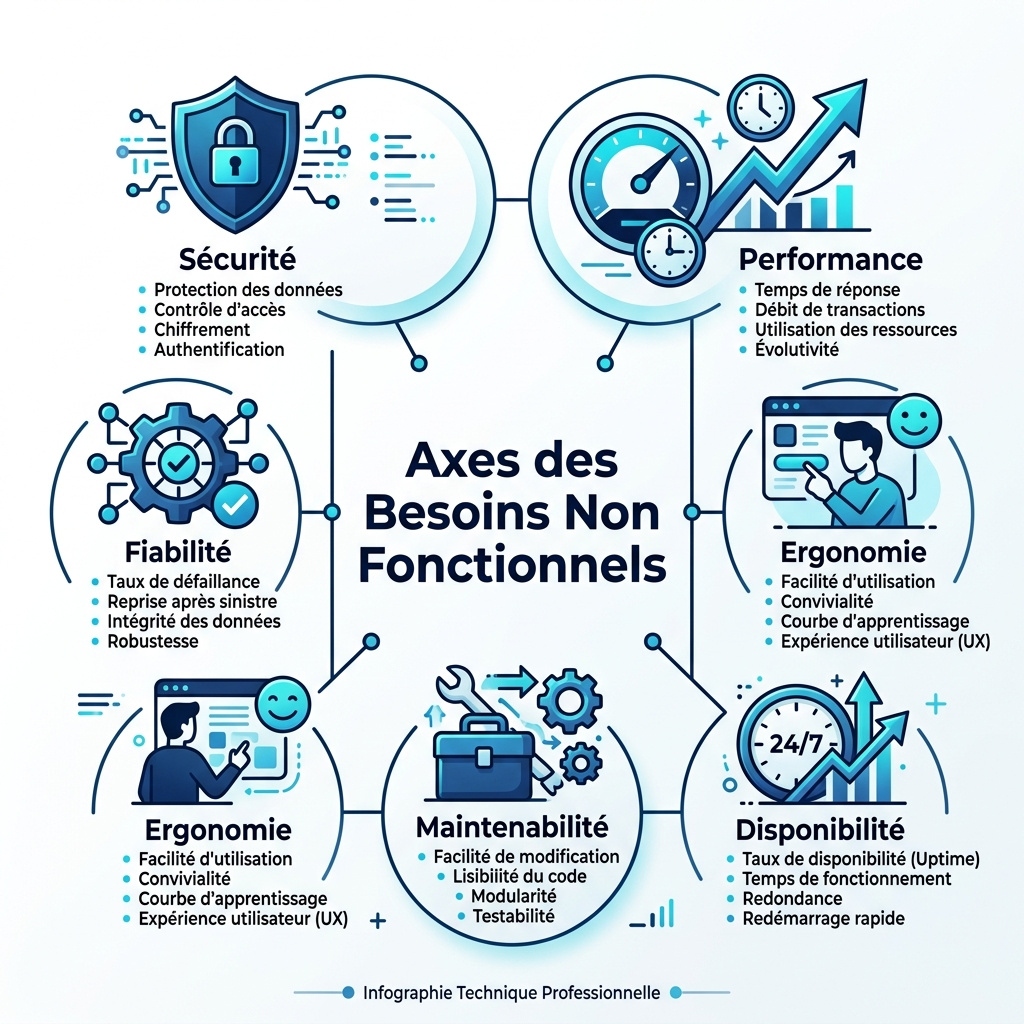
\includegraphics[width=0.7\textwidth]{IMAGE_BESOINS_NON_FONCTIONNELS.png}
%     \caption{Besoins non fonctionnels de StageFlow}
% \end{figure}

\section{Diagramme de cas d'utilisation global}
Le diagramme de cas d'utilisation global illustre les interactions entre les acteurs et les principales fonctionnalités du système.

%%% --- IMAGE : Diagramme de cas d'utilisation global ---
%%% Remplacer IMAGE_CAS_UTILISATION_GLOBAL.png par le nom de ton image
% \begin{figure}[H]
%     \centering
%     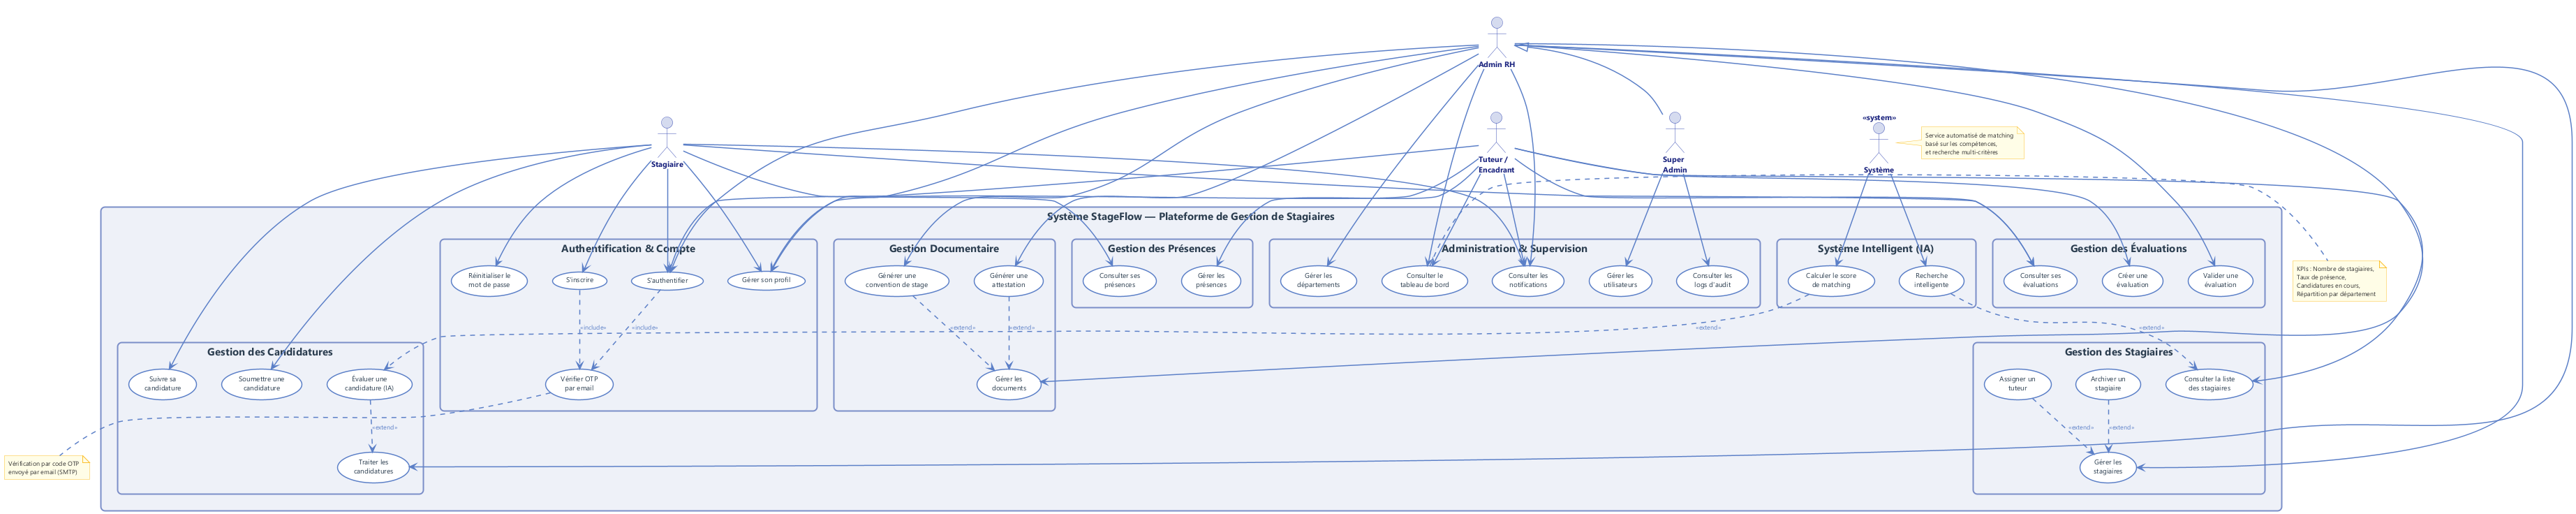
\includegraphics[width=0.85\textwidth]{IMAGE_CAS_UTILISATION_GLOBAL.png}
%     \caption{Diagramme de cas d'utilisation global de StageFlow}
% \end{figure}

Les principaux cas d'utilisation identifiés sont :
\begin{itemize}
    \item \textbf{S'inscrire et se connecter} : Accessible par tous les acteurs avec vérification par email.
    \item \textbf{Soumettre une candidature} : Le candidat remplit un formulaire et joint ses documents.
    \item \textbf{Gérer les candidatures} : L'Admin RH traite les dossiers reçus.
    \item \textbf{Gérer les stagiaires} : Affectation, suivi et encadrement des stagiaires.
    \item \textbf{Gérer les présences} : Saisie quotidienne par le tuteur.
    \item \textbf{Évaluer les stagiaires} : Le tuteur remplit une fiche d'évaluation.
    \item \textbf{Générer les documents} : Conventions et attestations en PDF.
    \item \textbf{Consulter le tableau de bord} : Statistiques et KPIs pour l'Admin RH.
\end{itemize}

\section{Diagramme de contexte statique}
Le diagramme de contexte statique positionne le système StageFlow dans son environnement et identifie les flux d'information échangés avec les acteurs externes.

%%% --- IMAGE : Diagramme de contexte statique ---
%%% Remplacer IMAGE_DIAGRAMME_CONTEXTE.png par le nom de ton image
% \begin{figure}[H]
%     \centering
%     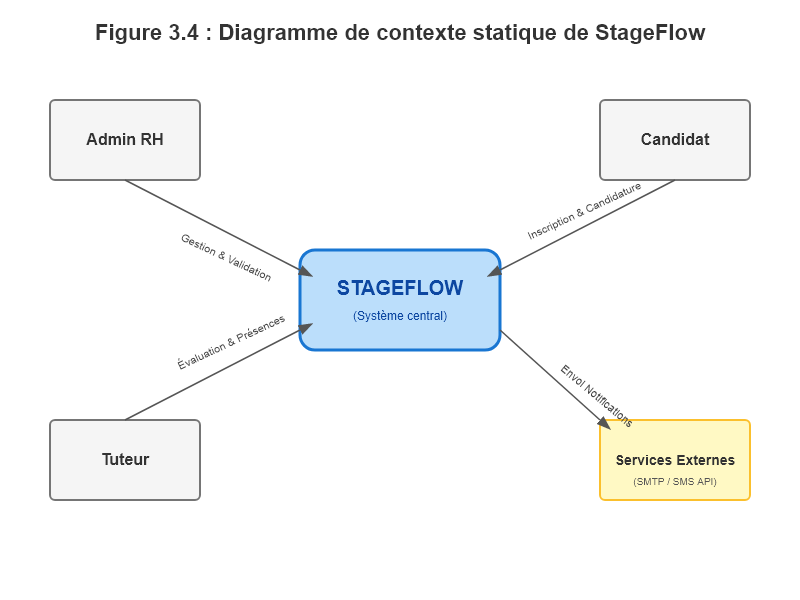
\includegraphics[width=0.8\textwidth]{IMAGE_DIAGRAMME_CONTEXTE.png}
%     \caption{Diagramme de contexte statique de StageFlow}
% \end{figure}

Les flux identifiés sont :
\begin{itemize}
    \item \textbf{Admin RH $\rightarrow$ StageFlow} : Gestion et validation des candidatures, affectation des stagiaires.
    \item \textbf{Candidat $\rightarrow$ StageFlow} : Inscription et candidature en ligne.
    \item \textbf{Tuteur $\rightarrow$ StageFlow} : Évaluations et présences des stagiaires.
    \item \textbf{StageFlow $\rightarrow$ Services Externes} : Envoi d'emails (SMTP) et notifications (SMS API).
\end{itemize}

\section{Product Backlog global}
Le Product Backlog regroupe l'ensemble des fonctionnalités à développer, organisées en sprints selon la méthodologie Scrum.

\begin{center}
\begin{tabular}{|l|p{6cm}|p{2cm}|p{3cm}|}
\hline
\textbf{Sprint} & \textbf{Objectif principal} & \textbf{Durée} & \textbf{Priorité} \\ \hline
\textbf{Sprint 0} & Mise en place de l'environnement et site vitrine & 2 semaines & Haute \\ \hline
\textbf{Sprint 1} & Authentification et gestion des utilisateurs & 2 semaines & Haute \\ \hline
\textbf{Sprint 2} & Gestion des candidatures et des départements & 3 semaines & Haute \\ \hline
\textbf{Sprint 3} & Gestion des présences et des évaluations & 2 semaines & Moyenne \\ \hline
\textbf{Sprint 4} & Conventions PDF, documents et notifications & 2 semaines & Moyenne \\ \hline
\end{tabular}
\captionof{table}{Product Backlog global de StageFlow}
\end{center}

\section{Conclusion}
Ce chapitre a permis de définir les besoins fonctionnels et non fonctionnels de la plateforme StageFlow. L'identification des acteurs et l'élaboration des diagrammes de cas d'utilisation et de contexte nous fournissent une vision claire du périmètre du système. Le Product Backlog global servira de feuille de route pour l'implémentation progressive des fonctionnalités au cours des sprints suivants.
